\documentclass[runningheads]{llncs}
\usepackage[newfloat]{minted}
\setminted[cpp]{
frame=lines,
linenos,
breaklines,
fontsize=\footnotesize,
framesep=2mm
}
\usepackage{caption}
\usepackage{graphicx}
\usepackage[portuguese]{babel}
\usepackage{hyphenat}
\usepackage{lscape}
\usepackage{microtype} % melhora a formatação do texto para evitar overfull box, entre outros
\usepackage{hyperref}
\usepackage{amsmath}
% to insert sourcecode
\newenvironment{code}{\captionsetup{type=listing}}{}
\SetupFloatingEnvironment{listing}{name=\underline{\textbf{CGDraw} Source Code}}

\begin{document}
%
\title{Relatório Computação Grafica - Fase 2}
\author{Marco Sousa\inst{1,2}\orcidID{62608} \and
    José Malheiro\inst{1,2}\orcidID{93271} \and
    Miguel Fernandes\inst{1,2}\orcidID{94269}}
%
\institute{Universidade do Minho\\
    \and Licenciatura em Engenharia Informática, Braga, Portugal}
%
\maketitle              % typeset the header of the contribution
%
\begin{abstract}
    Por forma a permitir a construção de um mundo gráfico virtual, é necessário 
    a possibilidade de transformações geométricas dos objetos a serem 
    construídos.
    Assim, procedeu-se à utilização das funções que permitem transformações geométricas,
    como glTranslate, glRotate e glScale para construir um modelo do sistema solar
    a partir da definição hierárquica do sol, planetas e luas.
    
    Procedeu-se, ainda, à utilização de VBO e implementação de uma câmera FPS para 
    navegar pelo mundo.
    
    \keywords{ OpenGL \and GLUT \and Glew \and c++ \and Transformations \and FPS}
\end{abstract}

\section{Introdução}

\subsection{Contextualização}

No seguimento da fase I do projeto da disciplina de \textit{Computação Gráfica} da Licenciatura em
Engenharia Informática da Universidade do Minho, foi proposto a aplicação de transformações geométricas
ao motor previamente desenvolvido, assim como o desenvolvimento de um modelo do sistema solar.

\subsection{Breve Descrição do Enunciado Proposto}
O principal foco da fase a que este relatório se remete é a aplicação de um conjunto de transformações geométricas,
tais como translação, rotação e escala de forma hierárquica a um conjunto de modelos.
Assim, a estrutura dos modelos é efetuada através da definição de grupos e respetivos subgrupos,
conforme exposto no enunciado.

Os grupos \textit{filhos} deverão adquirir as transformações geométricas dos \textit{pais},
i.e. as transformações são aplicados a todos os modelos e subgrupos.
As transformações geométricas devem ser aplicadas na mesma ordem que são definidas no ficheiro de \textit{input}.

Por último, foi proposto o desenvolvimento de um modelo \textbf{estático} do sistema solar, incluíndo o sol,
planetas e luas definidas de forma hierárquica.

\section{Trabalho Realizado}
Funcionalidades implementadas:
\begin{enumerate}
    \item Transformações geométricas aplicadas de forma hierárquica (\ref{sec:transf_geometricas})
          \begin{enumerate}
              \item Possibilidade de aplicar múltiplas vezes a mesma transformação
              \item Garantia de aplicação das transformações pela mesma ordem que a definida no ficheiro de \textit{input}
          \end{enumerate}
    \item Navegação com câmera $FPS$ (\ref{sec:camera_fps})
          \begin{enumerate}
              \item Acréscimo de escala de navegação
          \end{enumerate}
    \item Implementação de VBO's
    \item Construção do modelo do sistema solar (\ref{sec:modelo_ss})
\end{enumerate}

\subsection{Transformações Geométricas} \label{sec:transf_geometricas}
Como consequência da arquitetura definida na fase $I$, a implementação desta fase foi facilitada.
Em particular, para aplicar as transformações geométricas de forma hierárquica, optou-se
por criar uma nova \mintinline{cpp}{class Transform} que se pode encontrar ao nível da
\mintinline{cpp}{class Group}.
Ao implementar desta forma, permitiu que um conjunto de transformações fosse aplicada em todo
o \textit{scope} do \textbf{Grupo} (seja modelos ou subgrupos).
Assim, pode-se encontrar a $Transform$ ao nível do objeto Group:

\begin{code}
    \captionof{listing}{Group}
    \label{code:group_h}
    \inputminted[firstline=12, lastline=18]{cpp}{../../Group.h}
\end{code}

Nesta classe ($Transform$), a primeira abordagem apenas permitia que se tivesse uma transformação
de cada tipo, sendo estas aplicadas pela ordem: translação, rotação e escala.
Após uma análise mais detalhada do enunciado e mediante as dificuldades encontradas
na construção do modelo do \textit{sistema solar}, verificou-se que seria necessário
a \textit{\textbf{engine}} ser capaz de aplicar múltiplas transformações do mesmo tipo,
no mesmo conjunto de elementos e que a sua ordem de aplicação poderia ser diferente daquela
definida de forma estática.
Assim, procedeu-se à alteração da \mintinline{cpp}{class Transform} para albergar um
\mintinline{cpp}{std::vector<transformation>}.

\begin{code}
    \captionof{listing}{Transformation}
    \label{code:struct_transformation}
    \inputminted[firstline=17, lastline=21]{cpp}{../../Transform.h}
\end{code}

Em termos concretos, pode-se encontrar a estratégia utilizada
representada no seguinte diagrama de sequência na figura \ref{fig:seq_transf_geom}.
Em suma, consiste em chamar de forma recursiva o método \mintinline{cpp}{void draw()} ao longo
da hierarquia do Grupo, Modelo e Subgrupos.

\subsection{Câmera $FPS$} \label{sec:camera_fps}
Optou-se por implementar a câmera do tipo $FPS$.
A sua implementação consistiu em utilizar uma biblioteca ("cartesian") desenvolvida pelo grupo para facilitar os cálculos
sobre pontos $3D$.

Durante o \textit{parsing} do ficheiro $XML$:
\begin{enumerate}
    \item \mintinline{cpp}{set_camera_pos(X, Y, Z)} - define a posição onde a câmera se encontra,
    a partir do elemento \mintinline{xml}{<position x="X" y="Y" z="Z" />}
    \item \mintinline{cpp}{set_camera_lookat(X, Y, Z)} - define a direção da câmera,
    a partir do elemento \mintinline{xml}{<lookAt x="X" y="Y" z="Z" />}
    \begin{enumerate}
        \item Cria-se um vetor entre os pontos $lookat$ e $position$
        \item Efetua-se a normalizalização do vetor para que seja unitário
        \item Armazena-se em duas estruturas distintas o valor em cartesiano e em polar
        (este último) permite posteriormente oscilar os ângulos $\alpha$ e $\beta$ para movimentar a câmera.
    \end{enumerate}
    \item \mintinline{cpp}{set_camera_up(X,Y,Z)} - define a orientação do vetor vertical da câmera a partir do 
    elemento \mintinline{xml}{<up x="X" y="Y" z="Z" />}
\end{enumerate}

Após efetuar o \textit{parsing} do \textit{xml}, tem-se o estado inicial de navegação.
A partir deste, foi utilizado os métodos \mintinline{cpp}{move_camera(CAMenum t)} e
\mintinline{cpp}{move_lookat(double alpha, double beta)}.

A movimentação do $lookat$ consiste em incrementar o valor do $\alpha$ conforme o movimento do 
rato ao longo da janela.
Quanto ao primeiro - move\_camera(CAMenum) efetua um movimento para a frente, trás, direita e esquerda.
Em qualquer um dos casos, é utilizado o vetor $lookat$ multiplicado por um escalar para movimentar a posição da câmera.
No caso de movimentar para a esquerda e direita, como a referência é para onde a câmera está a olhar,
utilizou-se uma rotação de $\pm90\deg$ e, posteriormente, movimentou-se a câmera.
Ao utilizar o vetor $lookAt$ garante-se que o movimento é uniforme e congruente com a sua direção.

\textbf{Nota:} Atualmente esta funcionalidade encontra-se com um 
\textit{bug}. A primeira interação do rato com o ecrã gera uma pequena 
deslocação do \textit{lookat}. 
Após esta, encontra-se uma interação fluída do utilizador.

\subsection{\textit{Vertex Buffer Object} (VBO)}
Optou-se por implementar, desde já, a utilização de VBO's
para melhorar a performance da renderização.

A implementação foi efetuada ao nível da \mintinline{cpp}{class Model},
que representa a definição de um modelo do sistema e
implicou pequenas alterações, nomeadamente:
\begin{itemize}
    \item Remoção da variável de instância \_points que apontava para um \mintinline{cpp}{std::vector}
    \item Acréscimo de um \mintinline{cpp}{GLuint _buffer} para apontar para um buffer gerado na memória da placa gráfica
\end{itemize}

Após estas alterações, tratou-se de alocar um buffer na memória 
da placa gráfica e popular esse buffer com os pontos a serem desenhados,
ficando o índice do buffer disponível como variável de instância.
Este procedimento decorre durante o \textit{parsing} do 
documento XML e respetiva leitura dos pontos do modelo:

\begin{code}
\captionof{listing}{Gerar e popular VBO}
\label{code:vbo_gen}
\inputminted[firstline=46, lastline=48]{cpp}{../../Model.cpp}
\end{code}

Depois de ter o \textit{buffer} disponível, a sua renderização
ocorre durante a execução do método \mintinline{cpp}{_draw}:
\begin{code}
\captionof{listing}{Renderizar VBO}
\label{code:render_vbo}
\inputminted[firstline=73, lastline=75]{cpp}{../../Model.cpp}
\end{code}

\textbf{Futuramente}, na \underline{próxima fase}, pretende-se a implementação
de VBO's com índices, por forma a otimizar a \textit{performance}.

\subsection{Modelo do Sistema Solar} \label{sec:modelo_ss}
Conforme requisitado pela equipa docente, procedeu-se
à construção de um modelo do sistema solar utilizando a
sintaxe \textit{XML} previamente definida, assim como
as figuras geométricas geradas pela aplicação \textbf{generator}, desenvolvido na fase I.

Assim, a construção do modelo consistiu na criação, de 
forma hierárquica, do sol, planetas e algumas luas.

A principal dificuldade prendeu-se com a escolha de uma escala adequada.
Atendendo às grandes dimensões de diâmetro dos planetas e ainda maior distância entre estes,
foi necessário definir escalas diferentes para ambas as medidas.

A escala do diâmetro e distância do sol foi obtida através da fórmula:
\begin{align*}
    terra_{diametro}^{scale} & = 10 u \\
    planeta_{x}^{scale} &= \frac{terra_{diametro}^{scale} \cdot planeta_{x}^{real}}{terra_{diametro}^{real}} \\
    distancia_{x}^{scale} &= \frac{x^{scale}\cdot x^{distance}_{real}}{x_{diametro}^{real}} \cdot 500^{-1}
\end{align*}

Depois de definida a escala, a sua concretização foi relativamente linear.
Através da utilização da \textit{sphere} gerada no \textit{generator},
aliado ao poder da translação e \textit{scale}, permitiu que se construísse
os vários planetas na posição previamente calculada com a escala definida.

De salientar a utilização da figura geométrica \textbf{\textit{tórus}} para 
a representação dos anéis de saturno.

Em suma, foi construído um grupo que corresponde à origem, onde é definido o sol.
Posteriormente, há vários subgrupos que identificam cada um dos planetas.
Os planetas Terra e Marte têm, ainda, outros subgrupos que permitem a
criação das suas luas.
Optou-se por não representar as luas de outros planetas, atendendo à sua quantidade.
O facto de se ter representado o sistema solar de forma hierárquica, 
permite que, nas fases que se aproximam seja mais fácil a implementação 
de animações relacionadas com cada planeta e/ ou a totalidade do sistema solar. 

\begin{landscape}
    \begin{figure}
        \centering
        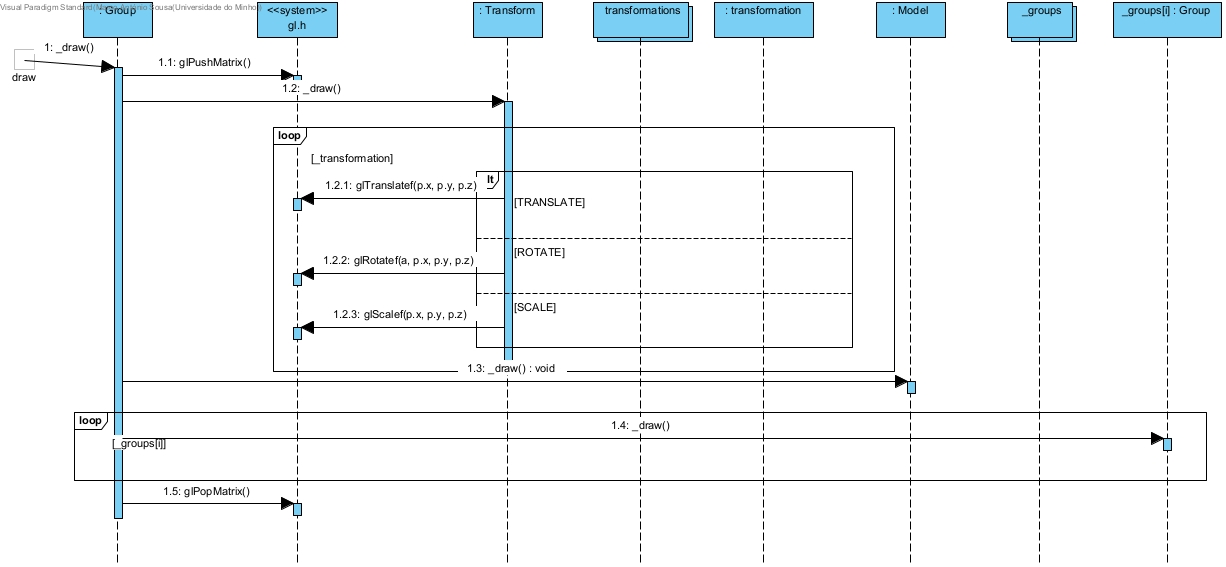
\includegraphics[width=\linewidth]{assets/geom_transf.jpg}
        \caption{Diagrama de sequência das transformações geométricas} \label{fig:seq_transf_geom}
    \end{figure}
\end{landscape}

\begin{landscape}
    \begin{figure}
        \centering
        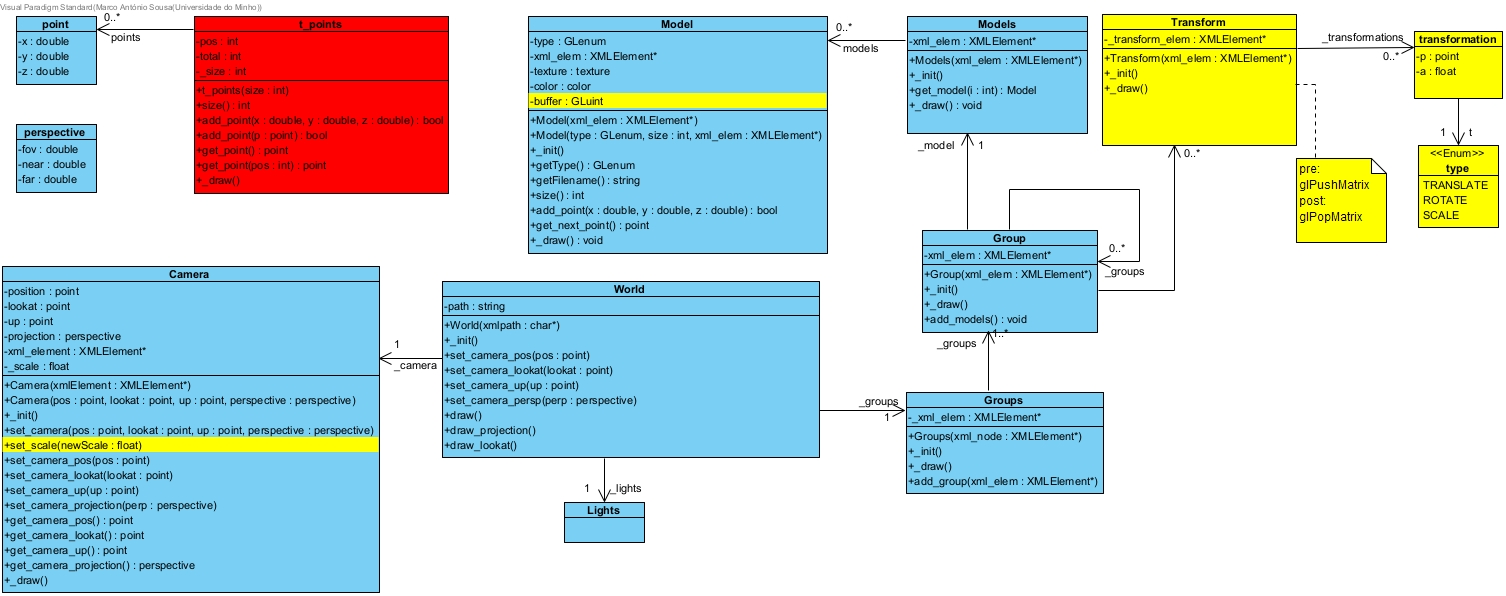
\includegraphics[width=\linewidth]{assets/world.jpg}
        \caption{Arquitetura da Aplicação - \textit{Alterações em relação à fase 1 a amarelo}.}
    \end{figure}
\end{landscape}

\section{Conclusão}
Com a conclusão da fase $I$, verificou-se que a implementação da atual fase 
se tornou bastante expedita pelo facto de se ter desenvolvido
uma arquitetura que permite a implementação de novas funcionalidades 
de forma quase \textit{cirúrgica}, i.e. é possível determinar o exato 
local onde se terá de efetuar alterações para que se obtenha o resultado
pretendido.

Assim, com a presente fase, foi possível implementar todos os requisitos 
definidos pela equipa docente e, ainda, acrescentar algumas funcionalidades extra.
Em particular, nesta fase foi implementado:
\begin{itemize}
    \item Transformações geométricas
    \item Geração do tórus
    \item Navegação com câmera FPS
    \item Utilização de VBO
    \item Construção do modelo do sistema solar
\end{itemize}

Assim, pretende-se na próxima fase implementar a utilização de VBOs 
com recurso a índices, tal como todas as funcionalidade propostas pela
equipa docente.

\section*{Anexos}
\subsection*{Modelo do Sistema Solar}
\begin{code}
\captionof{listing}{Modelo do Sistema Solar}
\label{code:sistema_solar_xml}
\inputminted[linenos, breaklines, frame=lines]{xml}{../../demos/solar_system.xml}
\end{code}


%
% ---- Bibliography ----
%
% BibTeX users should specify bibliography style 'splncs04'.
% References will then be sorted and formatted in the correct style.
%
% \bibliographystyle{splncs04}
% \bibliography{mybibliography}
%

\end{document}